% Created by tikzDevice version 0.12.6 on 2024-06-10 23:46:13
% !TEX encoding = UTF-8 Unicode
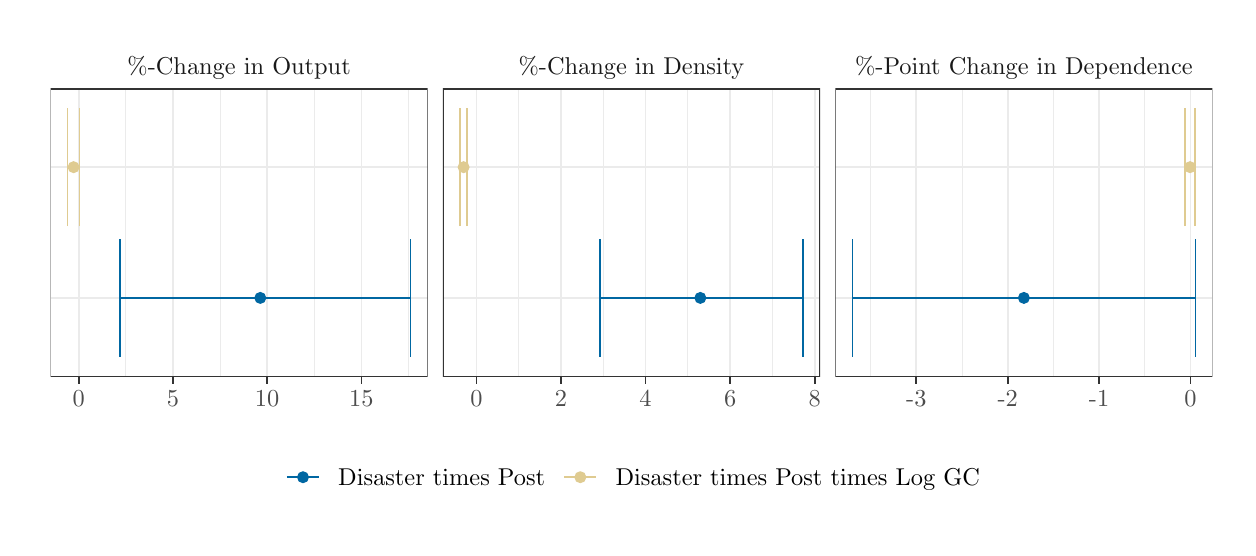
\begin{tikzpicture}[x=1pt,y=1pt]
\definecolor{fillColor}{RGB}{255,255,255}
\path[use as bounding box,fill=fillColor,fill opacity=0.00] (0,0) rectangle (433.62,180.67);
\begin{scope}
\path[clip] (  0.00,  0.00) rectangle (433.62,180.67);
\definecolor{drawColor}{RGB}{255,255,255}
\definecolor{fillColor}{RGB}{255,255,255}

\path[draw=drawColor,line width= 0.6pt,line join=round,line cap=round,fill=fillColor] (  0.00,  0.00) rectangle (433.62,180.68);
\end{scope}
\begin{scope}
\path[clip] (  8.25, 54.68) rectangle (144.54,158.60);
\definecolor{fillColor}{RGB}{255,255,255}

\path[fill=fillColor] (  8.25, 54.68) rectangle (144.54,158.60);
\definecolor{drawColor}{gray}{0.92}

\path[draw=drawColor,line width= 0.3pt,line join=round] ( 35.46, 54.68) --
	( 35.46,158.60);

\path[draw=drawColor,line width= 0.3pt,line join=round] ( 69.51, 54.68) --
	( 69.51,158.60);

\path[draw=drawColor,line width= 0.3pt,line join=round] (103.57, 54.68) --
	(103.57,158.60);

\path[draw=drawColor,line width= 0.3pt,line join=round] (137.62, 54.68) --
	(137.62,158.60);

\path[draw=drawColor,line width= 0.6pt,line join=round] (  8.25, 83.02) --
	(144.54, 83.02);

\path[draw=drawColor,line width= 0.6pt,line join=round] (  8.25,130.26) --
	(144.54,130.26);

\path[draw=drawColor,line width= 0.6pt,line join=round] ( 18.43, 54.68) --
	( 18.43,158.60);

\path[draw=drawColor,line width= 0.6pt,line join=round] ( 52.48, 54.68) --
	( 52.48,158.60);

\path[draw=drawColor,line width= 0.6pt,line join=round] ( 86.54, 54.68) --
	( 86.54,158.60);

\path[draw=drawColor,line width= 0.6pt,line join=round] (120.59, 54.68) --
	(120.59,158.60);
\definecolor{drawColor}{RGB}{0,103,162}
\definecolor{fillColor}{RGB}{0,103,162}

\path[draw=drawColor,line width= 0.4pt,line join=round,line cap=round,fill=fillColor] ( 84.06, 83.02) circle (  1.96);
\definecolor{drawColor}{RGB}{223,203,145}
\definecolor{fillColor}{RGB}{223,203,145}

\path[draw=drawColor,line width= 0.4pt,line join=round,line cap=round,fill=fillColor] ( 16.59,130.26) circle (  1.96);
\definecolor{drawColor}{RGB}{0,103,162}

\path[draw=drawColor,line width= 0.6pt,line join=round] (138.34, 61.76) --
	(138.34,104.28);

\path[draw=drawColor,line width= 0.6pt,line join=round] (138.34, 83.02) --
	( 33.45, 83.02);

\path[draw=drawColor,line width= 0.6pt,line join=round] ( 33.45, 61.76) --
	( 33.45,104.28);
\definecolor{drawColor}{RGB}{223,203,145}

\path[draw=drawColor,line width= 0.6pt,line join=round] ( 18.74,109.00) --
	( 18.74,151.52);

\path[draw=drawColor,line width= 0.6pt,line join=round] ( 18.74,130.26) --
	( 14.45,130.26);

\path[draw=drawColor,line width= 0.6pt,line join=round] ( 14.45,109.00) --
	( 14.45,151.52);
\definecolor{drawColor}{gray}{0.20}

\path[draw=drawColor,line width= 0.6pt,line join=round,line cap=round] (  8.25, 54.68) rectangle (144.54,158.60);
\end{scope}
\begin{scope}
\path[clip] (150.04, 54.68) rectangle (286.33,158.60);
\definecolor{fillColor}{RGB}{255,255,255}

\path[fill=fillColor] (150.04, 54.68) rectangle (286.33,158.60);
\definecolor{drawColor}{gray}{0.92}

\path[draw=drawColor,line width= 0.3pt,line join=round] (177.42, 54.68) --
	(177.42,158.60);

\path[draw=drawColor,line width= 0.3pt,line join=round] (207.99, 54.68) --
	(207.99,158.60);

\path[draw=drawColor,line width= 0.3pt,line join=round] (238.55, 54.68) --
	(238.55,158.60);

\path[draw=drawColor,line width= 0.3pt,line join=round] (269.11, 54.68) --
	(269.11,158.60);

\path[draw=drawColor,line width= 0.6pt,line join=round] (150.04, 83.02) --
	(286.33, 83.02);

\path[draw=drawColor,line width= 0.6pt,line join=round] (150.04,130.26) --
	(286.33,130.26);

\path[draw=drawColor,line width= 0.6pt,line join=round] (162.14, 54.68) --
	(162.14,158.60);

\path[draw=drawColor,line width= 0.6pt,line join=round] (192.70, 54.68) --
	(192.70,158.60);

\path[draw=drawColor,line width= 0.6pt,line join=round] (223.27, 54.68) --
	(223.27,158.60);

\path[draw=drawColor,line width= 0.6pt,line join=round] (253.83, 54.68) --
	(253.83,158.60);

\path[draw=drawColor,line width= 0.6pt,line join=round] (284.39, 54.68) --
	(284.39,158.60);
\definecolor{drawColor}{RGB}{0,103,162}
\definecolor{fillColor}{RGB}{0,103,162}

\path[draw=drawColor,line width= 0.4pt,line join=round,line cap=round,fill=fillColor] (243.07, 83.02) circle (  1.96);
\definecolor{drawColor}{RGB}{223,203,145}
\definecolor{fillColor}{RGB}{223,203,145}

\path[draw=drawColor,line width= 0.4pt,line join=round,line cap=round,fill=fillColor] (157.52,130.26) circle (  1.96);
\definecolor{drawColor}{RGB}{0,103,162}

\path[draw=drawColor,line width= 0.6pt,line join=round] (280.13, 61.76) --
	(280.13,104.28);

\path[draw=drawColor,line width= 0.6pt,line join=round] (280.13, 83.02) --
	(206.84, 83.02);

\path[draw=drawColor,line width= 0.6pt,line join=round] (206.84, 61.76) --
	(206.84,104.28);
\definecolor{drawColor}{RGB}{223,203,145}

\path[draw=drawColor,line width= 0.6pt,line join=round] (158.80,109.00) --
	(158.80,151.52);

\path[draw=drawColor,line width= 0.6pt,line join=round] (158.80,130.26) --
	(156.24,130.26);

\path[draw=drawColor,line width= 0.6pt,line join=round] (156.24,109.00) --
	(156.24,151.52);
\definecolor{drawColor}{gray}{0.20}

\path[draw=drawColor,line width= 0.6pt,line join=round,line cap=round] (150.04, 54.68) rectangle (286.33,158.60);
\end{scope}
\begin{scope}
\path[clip] (291.83, 54.68) rectangle (428.12,158.60);
\definecolor{fillColor}{RGB}{255,255,255}

\path[fill=fillColor] (291.83, 54.68) rectangle (428.12,158.60);
\definecolor{drawColor}{gray}{0.92}

\path[draw=drawColor,line width= 0.3pt,line join=round] (304.59, 54.68) --
	(304.59,158.60);

\path[draw=drawColor,line width= 0.3pt,line join=round] (337.61, 54.68) --
	(337.61,158.60);

\path[draw=drawColor,line width= 0.3pt,line join=round] (370.63, 54.68) --
	(370.63,158.60);

\path[draw=drawColor,line width= 0.3pt,line join=round] (403.65, 54.68) --
	(403.65,158.60);

\path[draw=drawColor,line width= 0.6pt,line join=round] (291.83, 83.02) --
	(428.12, 83.02);

\path[draw=drawColor,line width= 0.6pt,line join=round] (291.83,130.26) --
	(428.12,130.26);

\path[draw=drawColor,line width= 0.6pt,line join=round] (321.10, 54.68) --
	(321.10,158.60);

\path[draw=drawColor,line width= 0.6pt,line join=round] (354.12, 54.68) --
	(354.12,158.60);

\path[draw=drawColor,line width= 0.6pt,line join=round] (387.14, 54.68) --
	(387.14,158.60);

\path[draw=drawColor,line width= 0.6pt,line join=round] (420.16, 54.68) --
	(420.16,158.60);
\definecolor{drawColor}{RGB}{0,103,162}
\definecolor{fillColor}{RGB}{0,103,162}

\path[draw=drawColor,line width= 0.4pt,line join=round,line cap=round,fill=fillColor] (359.98, 83.02) circle (  1.96);
\definecolor{drawColor}{RGB}{223,203,145}
\definecolor{fillColor}{RGB}{223,203,145}

\path[draw=drawColor,line width= 0.4pt,line join=round,line cap=round,fill=fillColor] (420.02,130.26) circle (  1.96);
\definecolor{drawColor}{RGB}{0,103,162}

\path[draw=drawColor,line width= 0.6pt,line join=round] (421.93, 61.76) --
	(421.93,104.28);

\path[draw=drawColor,line width= 0.6pt,line join=round] (421.93, 83.02) --
	(298.03, 83.02);

\path[draw=drawColor,line width= 0.6pt,line join=round] (298.03, 61.76) --
	(298.03,104.28);
\definecolor{drawColor}{RGB}{223,203,145}

\path[draw=drawColor,line width= 0.6pt,line join=round] (421.84,109.00) --
	(421.84,151.52);

\path[draw=drawColor,line width= 0.6pt,line join=round] (421.84,130.26) --
	(418.21,130.26);

\path[draw=drawColor,line width= 0.6pt,line join=round] (418.21,109.00) --
	(418.21,151.52);
\definecolor{drawColor}{gray}{0.20}

\path[draw=drawColor,line width= 0.6pt,line join=round,line cap=round] (291.83, 54.68) rectangle (428.12,158.60);
\end{scope}
\begin{scope}
\path[clip] (  8.25,158.60) rectangle (144.54,175.17);
\definecolor{drawColor}{gray}{0.10}

\node[text=drawColor,anchor=base,inner sep=0pt, outer sep=0pt, scale=  0.88] at ( 76.40,163.86) {\%-Change in Output};
\end{scope}
\begin{scope}
\path[clip] (150.04,158.60) rectangle (286.33,175.17);
\definecolor{drawColor}{gray}{0.10}

\node[text=drawColor,anchor=base,inner sep=0pt, outer sep=0pt, scale=  0.88] at (218.18,163.86) {\%-Change in Density};
\end{scope}
\begin{scope}
\path[clip] (291.83,158.60) rectangle (428.12,175.17);
\definecolor{drawColor}{gray}{0.10}

\node[text=drawColor,anchor=base,inner sep=0pt, outer sep=0pt, scale=  0.88] at (359.98,163.86) {\%-Point Change in Dependence};
\end{scope}
\begin{scope}
\path[clip] (  0.00,  0.00) rectangle (433.62,180.67);
\definecolor{drawColor}{gray}{0.20}

\path[draw=drawColor,line width= 0.6pt,line join=round] ( 18.43, 51.93) --
	( 18.43, 54.68);

\path[draw=drawColor,line width= 0.6pt,line join=round] ( 52.48, 51.93) --
	( 52.48, 54.68);

\path[draw=drawColor,line width= 0.6pt,line join=round] ( 86.54, 51.93) --
	( 86.54, 54.68);

\path[draw=drawColor,line width= 0.6pt,line join=round] (120.59, 51.93) --
	(120.59, 54.68);
\end{scope}
\begin{scope}
\path[clip] (  0.00,  0.00) rectangle (433.62,180.67);
\definecolor{drawColor}{gray}{0.30}

\node[text=drawColor,anchor=base,inner sep=0pt, outer sep=0pt, scale=  0.88] at ( 18.43, 43.66) {0};

\node[text=drawColor,anchor=base,inner sep=0pt, outer sep=0pt, scale=  0.88] at ( 52.48, 43.66) {5};

\node[text=drawColor,anchor=base,inner sep=0pt, outer sep=0pt, scale=  0.88] at ( 86.54, 43.66) {10};

\node[text=drawColor,anchor=base,inner sep=0pt, outer sep=0pt, scale=  0.88] at (120.59, 43.66) {15};
\end{scope}
\begin{scope}
\path[clip] (  0.00,  0.00) rectangle (433.62,180.67);
\definecolor{drawColor}{gray}{0.20}

\path[draw=drawColor,line width= 0.6pt,line join=round] (162.14, 51.93) --
	(162.14, 54.68);

\path[draw=drawColor,line width= 0.6pt,line join=round] (192.70, 51.93) --
	(192.70, 54.68);

\path[draw=drawColor,line width= 0.6pt,line join=round] (223.27, 51.93) --
	(223.27, 54.68);

\path[draw=drawColor,line width= 0.6pt,line join=round] (253.83, 51.93) --
	(253.83, 54.68);

\path[draw=drawColor,line width= 0.6pt,line join=round] (284.39, 51.93) --
	(284.39, 54.68);
\end{scope}
\begin{scope}
\path[clip] (  0.00,  0.00) rectangle (433.62,180.67);
\definecolor{drawColor}{gray}{0.30}

\node[text=drawColor,anchor=base,inner sep=0pt, outer sep=0pt, scale=  0.88] at (162.14, 43.66) {0};

\node[text=drawColor,anchor=base,inner sep=0pt, outer sep=0pt, scale=  0.88] at (192.70, 43.66) {2};

\node[text=drawColor,anchor=base,inner sep=0pt, outer sep=0pt, scale=  0.88] at (223.27, 43.66) {4};

\node[text=drawColor,anchor=base,inner sep=0pt, outer sep=0pt, scale=  0.88] at (253.83, 43.66) {6};

\node[text=drawColor,anchor=base,inner sep=0pt, outer sep=0pt, scale=  0.88] at (284.39, 43.66) {8};
\end{scope}
\begin{scope}
\path[clip] (  0.00,  0.00) rectangle (433.62,180.67);
\definecolor{drawColor}{gray}{0.20}

\path[draw=drawColor,line width= 0.6pt,line join=round] (321.10, 51.93) --
	(321.10, 54.68);

\path[draw=drawColor,line width= 0.6pt,line join=round] (354.12, 51.93) --
	(354.12, 54.68);

\path[draw=drawColor,line width= 0.6pt,line join=round] (387.14, 51.93) --
	(387.14, 54.68);

\path[draw=drawColor,line width= 0.6pt,line join=round] (420.16, 51.93) --
	(420.16, 54.68);
\end{scope}
\begin{scope}
\path[clip] (  0.00,  0.00) rectangle (433.62,180.67);
\definecolor{drawColor}{gray}{0.30}

\node[text=drawColor,anchor=base,inner sep=0pt, outer sep=0pt, scale=  0.88] at (321.10, 43.66) {-3};

\node[text=drawColor,anchor=base,inner sep=0pt, outer sep=0pt, scale=  0.88] at (354.12, 43.66) {-2};

\node[text=drawColor,anchor=base,inner sep=0pt, outer sep=0pt, scale=  0.88] at (387.14, 43.66) {-1};

\node[text=drawColor,anchor=base,inner sep=0pt, outer sep=0pt, scale=  0.88] at (420.16, 43.66) {0};
\end{scope}
\begin{scope}
\path[clip] (  0.00,  0.00) rectangle (433.62,180.67);
\definecolor{fillColor}{RGB}{255,255,255}

\path[fill=fillColor] ( 86.76,  5.50) rectangle (349.61, 30.95);
\end{scope}
\begin{scope}
\path[clip] (  0.00,  0.00) rectangle (433.62,180.67);
\definecolor{fillColor}{RGB}{255,255,255}

\path[fill=fillColor] ( 92.26, 11.00) rectangle (106.71, 25.45);
\end{scope}
\begin{scope}
\path[clip] (  0.00,  0.00) rectangle (433.62,180.67);
\definecolor{drawColor}{RGB}{0,103,162}
\definecolor{fillColor}{RGB}{0,103,162}

\path[draw=drawColor,line width= 0.4pt,line join=round,line cap=round,fill=fillColor] ( 99.49, 18.23) circle (  1.96);
\end{scope}
\begin{scope}
\path[clip] (  0.00,  0.00) rectangle (433.62,180.67);
\definecolor{drawColor}{RGB}{0,103,162}

\path[draw=drawColor,line width= 0.6pt,line join=round] ( 93.70, 18.23) -- (105.27, 18.23);
\end{scope}
\begin{scope}
\path[clip] (  0.00,  0.00) rectangle (433.62,180.67);
\definecolor{fillColor}{RGB}{255,255,255}

\path[fill=fillColor] (192.47, 11.00) rectangle (206.92, 25.45);
\end{scope}
\begin{scope}
\path[clip] (  0.00,  0.00) rectangle (433.62,180.67);
\definecolor{drawColor}{RGB}{223,203,145}
\definecolor{fillColor}{RGB}{223,203,145}

\path[draw=drawColor,line width= 0.4pt,line join=round,line cap=round,fill=fillColor] (199.70, 18.23) circle (  1.96);
\end{scope}
\begin{scope}
\path[clip] (  0.00,  0.00) rectangle (433.62,180.67);
\definecolor{drawColor}{RGB}{223,203,145}

\path[draw=drawColor,line width= 0.6pt,line join=round] (193.92, 18.23) -- (205.48, 18.23);
\end{scope}
\begin{scope}
\path[clip] (  0.00,  0.00) rectangle (433.62,180.67);
\definecolor{drawColor}{RGB}{0,0,0}

\node[text=drawColor,anchor=base west,inner sep=0pt, outer sep=0pt, scale=  0.88] at (112.21, 15.20) {Disaster times Post};
\end{scope}
\begin{scope}
\path[clip] (  0.00,  0.00) rectangle (433.62,180.67);
\definecolor{drawColor}{RGB}{0,0,0}

\node[text=drawColor,anchor=base west,inner sep=0pt, outer sep=0pt, scale=  0.88] at (212.42, 15.20) {Disaster times Post times Log GC};
\end{scope}
\end{tikzpicture}
